\documentclass[12pt,a4paper,twoside]{report}

\usepackage[utf8]{inputenc}
\usepackage[margin=1in]{geometry}
\usepackage{setspace}
\usepackage{fancyhdr}
\usepackage{natbib}
\usepackage{hyperref}
\usepackage{setspace}
\usepackage{etoolbox}
\usepackage{endnotes}
\usepackage{graphicx}
\usepackage[labelfont=it]{caption}
\usepackage{lscape}
\usepackage{ array, blindtext}
\usepackage{tabularx,ragged2e,booktabs}
\usepackage[export]{adjustbox}
\usepackage{soul}
\usepackage{pifont}
\usepackage[section]{placeins}


\newcolumntype{C}[1]{>{\Centering}m{#1}}
\renewcommand\tabularxcolumn[1]{C{#1}}

\let\footnote=\endnote

\makeatletter
\pretocmd{\@sect}{\singlespacing}{}{}
\pretocmd{\@ssect}{\singlespacing}{}{}
\apptocmd{\@sect}{\doublespacing}{}{}
\apptocmd{\@ssect}{\doublespacing}{}{}
\makeatother

\hypersetup{
	colorlinks,
	citecolor=black,
	filecolor=black,
	linkcolor=black,
	urlcolor=black
}


\makeatletter
\def\@makechapterhead#1{%
	\singlespacing
	\vspace*{30\p@}%
	{\parindent \z@ \raggedright \normalfont
		\interlinepenalty\@M
		\huge\bfseries  \thechapter.\quad #1\par\nobreak
		\vskip 20\p@
}
\doublespacing
}
\makeatother

\begin{document}

%front matter
\pagenumbering{gobble}
\begin{titlepage}
	\centering
	\vspace{1cm}
	{\scshape\Large McGill University\par}
	\vspace{1.5cm}
	{\huge\bfseries On the\\Automated Regional Classification\\of Early Breast Cancers\par}
	\vspace{2cm}
	{\Large\itshape Joseph Szymborski\par}
	\vspace{1cm}
	{\large Faculty of Medicine\\
		Division of Experimental Medicine\\
		McGill University, Montréal\\
		September, 2017\par}
	\vspace{1.5cm}
	Supervised by:\par
	Prof.~Luke M. \textsc{McCaffrey}
	
	\vfill
	{A thesis submitted to McGill University in partial fulfilment\\of the requirements of the Master's degree.\par}
	\vfill

% Bottom of the page
	{© Joseph Szymborski, 2017\par}
	%{\large \today\par}
\end{titlepage}

\pagenumbering{roman}
\newpage
\section*{Abstract}
\addcontentsline{toc}{section}{Abstract}

The harbinger of a far more lethal and difficult-to-treat disease, 
early breast cancer is a key, but often overlooked, point of study. 
Early breast cancers are often difficult to detect and classify, and 
the subjective nature of the histopathological methods used to detect 
them often result in dissenting diagnoses between clinicians. These 
issues can be mitigated through the use of quantitative computational 
methods, although existing solutions do not account for the 
heterogeneity of tumours, and often do not operate in manner that is
transparent to the clinician; precluding their utility in a clinical 
setting.

This work presents two models which address the concerns of tumour 
intraheterogeneity by detecting, classifying and annotating regions 
within fields of breast biopsy sections that appear to belong to early 
lesions. The PPReCOGG model, which is a GPU-accelerated texture-based 
classifier, is able to generate pixel-resolution annotations of cell-patterning
that is characteristic of early lesions with robust accuracy 
($\approx94.3\%$ average accuracy in synthetic benchmarks). DeepDuct 
is a deep learning model that provides accurate and transparent 
localisation and classification of lesions using gradient-based class 
activation maps (Grad-CAM). These two models illustrate that it is 
possible to develop clinically relevant classifiers that can achieve 
robust accuracy and account for tumour heterogeneity and model 
transparency.
\newpage
\section*{Résumé}
\addcontentsline{toc}{section}{Résumé}
\newpage
\section*{Acknowledgements}
\addcontentsline{toc}{section}{Acknowledgements}
\newpage
\section*{Abbreviations}
\addcontentsline{toc}{section}{Abbreviations}
\newpage
\section*{Preface}
\addcontentsline{toc}{section}{Preface}

%% NOTE
%% The preface needs to entirely revised. This is more of a place-holder than anything else. I might just not include an overview, but the idea was to unite the disperate chapters and with a theme and set the overall tone.

\subsection*{Overview}
\addcontentsline{toc}{subsection}{Overview}
The harbinger of a far more lethal and difficult-to-treat disease, early breast cancer is a key, but often overlooked, point of study. Early breast cancers are often difficult to detect and classify, and the mode of progression between pre-invasive breast cancer lesions is not entirely understood.\par

Through the development of computational models for the regional detection and classification of early breast cancers, and by characterising the role of tight-junctions in their progression through traditional molecular biology; the projects herein offer novel insight into the fundamental nature of pre-invasive lesions of the mammary gland.\par
 
\subsection*{Contributions}
\addcontentsline{toc}{subsection}{Contributions}
\subsection*{Funding}
\addcontentsline{toc}{subsection}{Funding}

\onehalfspacing
\tableofcontents
\pagenumbering{gobble}

\pagestyle{fancy}
\fancyhead[LE,RO]{}
\fancyhead[RE,LO]{\it\rightmark}
\fancyfoot[CE,CO]{}
\fancyfoot[LE,RO]{\thepage}
\renewcommand{\footrulewidth}{0.5pt}

%main matter
\doublespacing
\pagenumbering{arabic}
%introduction

\newpage
\chapter{Introduction}
\section{An Anatomy of Early Breast Cancers}
Breast cancer is both a common and lethal diseases, having earned the dubious distinction of being both the most common and second most fatal cancer amongst females in Canada and around the world \citep{ccs2015}. Breast cancer most commonly arises in the epithelium of the mammary gland's many lactiferous ducts, which form a network that delivers to the nipple the milk that is secreted by the lobules of the mammary gland; which is another origin of breast carcinomas. The epithelium of the lactiferous duct is highly organised, with well-defined tissue and cell polarity that is integral to the structure and function of the duct. The tube-like lactiferous duct is a bilayered structure comprised of the outer myoepithelial and inner epithelial monolayers, both surrounding a hollow lumen at the duct's core. This epithelial inner-layer is surrounded by an outer layer of myoepithelial cells which express smooth-muscle actin (SMA) whose muscle-like contractile properties biomechanically deliver milk along the duct in response to hormonal signal \citep{Hamperl_1970}.\par

%NOTE: Will add a diagram illustrating the mammary gland, and the structure of the ducts and lobules

\subsection{Stages of Early Breast Cancer Progression}
When diagnosing a suspected early breast cancer, pathologists analyse needle-core biopsies with the aim of identifying and classifying any lesions that may be present. Classification of lesions allow medical professionals to better understand the nature of the particular disease, what treatment is most appropriate, and what statistical outcomes are associated with the lesion.\par

The early stages of breast cancer manifest as pre-invasive, hyper-proliferative lesions that exhibit progressive and gradual deterioration of this epithelial organisation. Of these lesions, there are four histologically distinct classes: Usual Hyperplasia (UH), Flat Epithelial Atypia (FEA), Atypical Ductal Hyperplasia (ADH) (or Atypical Lobular Hyperplasia [ALH] when referring to the less common lobular lesion), and Ductal Carcinoma {\it In Situ} (DCIS).\par

Ductal or lobular hyperplasias that do not present with abnormal tissue architecture or dysplasia are classified as Usual Hyperplasia (UH), or alternatively Proliferative Disease without Atypia (PDWA). These lesions confer a relative risk of later developping breast cancer as high as 1.9, although this increase in risk is not considered sufficient to warrant any prophylactic measures, including increased follow-up \citep{mommers2001}. While UH is traditionally believed to progress serially through ADH, DCIS and ultimately IDC due to early Loss of Homozygosity (LOH) analysis, more recent cytokeratin immunophenotype and genetic hybridisation analysis has contested the evolutionary relationship between UH and other proliferative breast lesions \citep{oconnell1994, boecker2002}.\par

ADH lesions are neoplasias of the lactiferous duct that exhibit subtle dysplasia (as evidenced by nuclear hyperchromaticity), and can form micropapillary or cribiform patterns \citep{page1959,dion2016}. Of the estimated one million instances of benign breast cancer detected in the USA each  year, 10\% are classified as ADH \citep{simpson2009}. While  these lesions have been long-known and extensively proven to impart a low relative risk (approximately 4), recent long-term follow-up studies have shown that one in eight individuals will develop more advanced (local or invasive) breast cancers ten years after their diagnosis. This proportion increases to 46\% in individuals with more than one atypical foci twenty-five years after diagnosis \citep{hartmann2015}.\par

Arising in the terminal duct-lobule unit of the breast, FEA lesions are a purported precursor to early low-grade ductal carcinomas, and in this regard are similar to ADH. Unlike ADH however, FEA lesions are far-more uncommon, never present with complex architectural patterns (thus the indication ``flat''), and are characterised by multi-layered dilated ascini often made-up of columnar cells \citep{pinder2017}. While ADH is suspected to arise from FEA lesions due their frequent coincidence, FEA is not independently associated with a long-term increased risk of breast cancer, leaving the matter unclear \citep{bombonati2011,lerwill2008,acott2016}.

%
% [ X ] poorly differentiated = >60% chance of recurrence (badve)
% [ X ] 500% increase of DCIS occurrence between 1983 to 2003 (kerlikowske)
% [   ] minor decrease in 10-year recurrence (21%-14%)
% - Surgery-Only 10yr (26%-19), Surgery+RTx (13%-11%); '78-'10 (Subhedar)
% [ X ] SMR after DCIS diagnosis is avg 1.8 (narod)
% [ X ] 30%-40% reoccur with invasive (Page, Betsill)
%


Benign early lesions go on to progress into localised malignant disease, which in the lactiferous duct is termed ductal carcinoma {\it in situ} (DCIS). DCIS is classified as a Stage 0 cancer and accounts for 20\% of all diagnosed breast cancers in the USA in 2003; representing a 500\% increase in occurrence over 20 years \citep{bleicher2013, kerlikowske2010}.\par

While DCIS has a relatively low average standardised mortality ratio (SMR) of 1.8, an estimated 30-50\% of cases reoccur as invasive breast cancers \citep{narod2015,page1982,betsill1978}. When further stratified by how well the lesion is differentiated, individuals with lesions classified as poorly differentiated (using the European Pathologists Working Group guidelines) have recurrence rates above 60\% \citep{badve1998}. At this early stage of cancer progression, the apical domain of the lumenal epithelium has begun to shrink, resulting in abnormally small lumen (a phenotype referred to as ``lumenal collapse'' herein). Our understanding of the processes by which transformed mammary duct epithelium undergoes lumenal collapse is still developing, but recent studies have described a mechanism by which lumenal tension is lost as myosin II and RhoA activity is greatly decreased at the lumenal membrane of DCIS lesions (Halaoui et al. 2017, in review). \par

The lesion becomes an invasive ductal carcinoma (IDC, or ILC in the lobular instances) when epithelial cells breach the surrounding myoepithelial layer of the duct and infiltrate into extra-cellular matrix (ECM). By this stage, cellular polarity is entirely disrupted and the apical membrane domain has completely disappeared.\par


\chapter{The Role of Tight-Junctions on the Early Progression of Breast Cancer}
\section{Introduction}
%    - What does polarity mean in lactiferous ducts?
%    - What macromolecules are involved?
%    - What processes does polarity regulate?

Loss of cellular organisation and polarity is a common feature across epithelial cancers, but unlike some other cancers like those that present in the colon where cell polarity is lost at late stages of the disease, loss of polarity is a hallmark of early breast cancer \citep{hinck2014}. The mechanisms by which epithelial cell polarity is lost in carcinomas, however, remains elusive and poorly understood.\par

When discussing the epithelial polarity of the lactiferous duct, one may be referring to asymmetric distribution at either the intercellular or intracellular level.\par

At the macro, intercellular scale, ductal epithelia is said to exhibit tissue polarity when cells organise into a monolayer forming a single lumen \citep{bissell2003}.\par

On the other hand, establishment of cellular apical-basolateral polarity is achieved by the intracellular asymmetric distribution of macromolecules within the inner epithelial monolayer of the mammary duct.

\subsection{Apical Polarity Proteins Complexes in Breast Cancers}

%        - [*] Crumbs complex proteins
%        - [ ] Crumbs3 & TJs (PATJ/Pals1)
%        - [*] FERM domain partners
%            - [*] Expandable/FRMD6
%            - [*] Yurt/Ehm2
%        - [*] Density sensing & Hippo (Not via FERM proteins)
%        - [ ] Crb3 homophilic interactions
%        - [ ] Pals1/Par6/aPKC & migration direction
%            - [ ] http://embor.embopress.org.proxy3.library.mcgill.ca/content/8/2/158
%            - [ ] http://www.sciencedirect.com/science/article/pii/S0092867402012497
%        - [ ] ZEB/Snail/Crb3 and EMT
%        - [ ] Crb3 homologues and isoforms?
%
% READ-UP ON STATEMENT:
% Might be tie-in to Ruba's paper?
% "The Ehm2/p114RhoGEF module organizes the circumferential actomyosin belt by
% activating RhoA and its effector kinases ROCK1 and ROCK2 (ROCK1/2)."
% doi: 10.1128/MCB.00673-15
%
% Nakajima H, Tanoue T. 2010. Epithelial cell shape is regulated by Lulu proteins
% via myosin-II. J Cell Sci 123: 555–566. http://dx.doi.org/10.1242/jcs.057752.
%
% Nakajima H, Tanoue T. 2012. The circumferential actomyosin belt in epithelial
% cells is regulated by the Lulu2-p114RhoGEF system. Small GTPases 3: 91–96.
% http://dx.doi.org/10.4161/sgtp.19112
%
% Terry SJ, Zihni C, Elbediwy A, Vitiello E, Leefa Chong San IV, Balda MS,
% Matter K. 2011. Spatially restricted activation of RhoA signalling at epithelial
% junctions by p114RhoGEF drives junction formation and morphogenesis.
% Nat Cell Biol 13:159–166. http://dx.doi.org/10.1038/ncb2156
%
% Nakajima H, Tanoue T. 2011. Lulu2 regulates the circumferential acto-myosin
% tensile system in epithelial cells through p114RhoGEF. J Cell Biol 195: 245–261.
% http://dx.doi.org/10.1083/jcb.201104118

Two protein complexes, the Crumbs complex and the Par complex, are particularly important determinants of the apical identity and play significant roles in the early progression of breast cancer \citep{horikoshi2009,whiteman2014}.\par

\subsubsection{The Crumbs Complex}
Localisation of the Crumbs complex to the plasma membrane both contributes to
the establishment and maintenance of its apical identity. The Crumbs complex
converges upon the apical transmembrane glycoprotein for which it is named,
Crumbs3 ({\it Crb3}), which serves as a scaffold for the complex. Crumbs3 directly
binds two proteins via its carboxy-terminal PDZ domain ({\tt ERLI}): protein
associated with {\it Lin-7} one (Pals1) and partitioning-defective protein six (Par6) \citep{lemmers2004, roh2002}.The presence of Pals1 also brings to the Crumbs complex the Pals1 associated tight junction (PATJ) protein, which is essential for proper polarisation and contributes to the establishment of tight-junctions in mammalian cells \citep{shin2005}.\par

% Insert Crb3 and TJs...

Crumbs3 has also been known to interact with FERM (4.1 protein, ezrin,
radixin and moesin) domain proteins through its PDZ domain. Crumbs3 also
interacts with the FERM-domain proteins EHM2 (also known as Lulu2) and YMO1,
homologues of {\it Drosophila melanogastor} protein Yurt, which helps to establish
apical-basolateral polarity and maintain the size of the apical membrane by
regulating Crumbs3 \citep{laprise2006}. Crumbs3 has also
been shown to recruit EHM2 and p114RhoGEF to maintain the actomyosin belt and
promote cell-cell adhesion in a cancer cell-lines, requiring both the C-terminal
FERM-binding and PDZ-binding motifs of Crumbs3 \citep{loie2015}.\par

The crumbs complex has been also shown to regulate important proliferative
programmes such as organ growth and mammary gland contact inhibition through the
Salvador/Warts/Hippo (hereafter Hippo) signalling pathway. Crumbs3 regulates the
Hippo pathway through interactions with, among other proteins, the FERM
domain-containing protein 6 ({\it FRMD6}), a mammalian homologue of the
{\it D. melanogastor} gene {\it Ex} \citep{robinson2010}. Crumbs3
also regulates the Hippo pathway through direct interaction with WW-domain proteins.
One such instance is the direct interaction between the Hippo pathway co-effectors
yes-associated protein 1 (YAP1), Tafazzin (TAZ), and Crumbs3; this occurs in
response to changes in cell density, which require changes to the cells
proliferative program \citep{varelas2010,szymaniak2015}. In a similar, cell-density-sensing
manner, Crumbs3 interacts directly with Kibra's WW-domain to stabilise it,
preventing its degradation and promoting Hippo-pathway-mediated proliferation
\citep{moleirinho2013,mao2017}.\par

Cell density is also coupled with transforming growth factor-$\beta$ (TGF-$\beta$)-induced
epithelial-mesenchymal transition (EMT) through the Crumbs3-mediated inhibition
of SMAD; effectively reducing downstream activation Snail
\citep{varelas2010}. In addition to being an important to the
EMT transcriptional programme, the zinc-finger protein Snail ({\it SNAI1}) is a potent
transcriptional inhibitor of Crumbs3 and to a lesser extent, PATJ and PALS1;
resulting in mislocalisation of the Crumbs and Par complexes and disruption of
tight-junction and polarity formation \citep{wang2013, whiteman2014}.\par

\subsubsection{The Par Complex}
The Par complex is named after the eponymous family of proteins first
discovered in the 1980s as part of screen to identify maternal effect lethal
mutations in the model nematode {\it Caenorhabditis elegans}
\citep{kemphues1988,goldstein2007}.
Of the six, the par proteins most relevant to apical membrane specification are
Par3 and Par6; both PDZ-domain scaffolding proteins and core members of the Par
complex \citep{yu2014,hung1999}. Other
members of the Par complex include atypical protein kinase C (aPKC) and the
cell division control protein 42 homologue (Cdc42) GTPase, binding to Par3
through Par6 which here acts as an adaptor \citep{joberty2000}.
Par3 is also capable of binding aPKC directly; an interaction that is essential
to establishing proper cell polarity, normal ductal architecture, and mammary
gland morphogenesis \citep{nagai2002, mccaffrey2009}.\par

The formation of the Par complex is cued by the establishment of cell-cell
contacts. This comes as a result of the complex being anchored to the tight-
junctions of the cell by Par3, which is tethered through its binding of
phosphotidyl inositols and the junctional adhesion molecule (JAM) through the
second and first of Par3s three PDZ domains, respectively \citep{wu2007,ebnet2001}.\par

At their basal levels of expression, the members of the Par complex are at a
regulatory equilibrium that is often disrupted in neoplasias, resulting in
aberrant signal integration and epithelial disorganisation. Human breast
cancers often express dramatically reduced levels of Par3, freeing aPKC to
inappropriately activate signalling pathways that lead to increased invasive and
metastatic potential; namely the human epidermal growth factor receptor 2 (HER2)
and janus kinase/two Signal Transducer and Activator of Transcription (JAK/STAT)
pathways \citep{xue2013,mccaffrey2012}.\par

aPKC is but one member of the mammalian Protein Kinase C (PKC) super family, of
which there are three additional members: the classical/conventional PKCs
(cPKCs), the novel PKCs (nPKCs), and the later-discovered PKC-related kinases
(PRKs). These families are distinguished by their dependence/independence
on $\textrm{Ca}^{2+}$, and whether they are activated by diacylglycerols (DAGs). aPKC is both $\textrm{Ca}^{2+}$-independent and DAG-insensitive, and in this respect are identical to PRKs.
The two families are primarily differentiated by PRKs association with RhoA,
which is unique among the PKCs \citep{mellor1998}.\par

Each PKC sub-family contains multiple isoforms, which each confer their own
unique function. The aPKC exists in two isoforms, aPKC$\lambda$/$\iota$ and aPKC$\zeta$.\par

\section{Materials \& Methods}
\section{Results}
\section{Discussion}
\chapter*{Preface}
\addcontentsline{toc}{chapter}{Preface}

\chapter{PPReCOGG: A Model for the Per-Pixel Classification of Early Breast Lesions via Gabor Features}

\section{Introduction}

When diagnosing breast cancer lesions, trained clinical pathologists rely on
visual interpretation of patient biopsies. While interobserver variability
between trained pathologists is a known problem, it is particularly pronounced
when pathologists are called to make distinction between early breast cancer
lesion stages \citep{gomes2014}.\par

Computer-aided detection (CADe) is sometimes used to enhance
interpretation of imaging from screening mammographies and can help manage the
ambiguous and subjective nature of medical imaging; however computational models
are not currently used in most clinical settings to assist the diagnosis of breast
cancers.\par

Despite many being described in the literature, a major limitation of most breast
cancer classification models is that they fail to model intra-tumour heterogeneity
as they commonly adopt whole-field classification modalities \citep{pareja2017,weigelt2010}. Whole-field classification models similarly do
not offer insight into so-called ``borderline'', which are lesions containing regions exhibiting features of multiple early lesions \citep{masood2011}.\par

To account for borderline lesions and the heterogeneous nature of cancer, a practical model for the classification of early lesions would be required to classify sub-regions of whole sections. As the characteristic ``cobblestone'' epithelial phenotype is altered distinctly
in the early progression of breast cancers, such a model would benefit from leveraging features which are based on differences in cell patterning.\par

The observation that early lesions exhibit distinct cell patterning unique to themselves are reported in the first descriptions of hyperplasia and carcinoma \textit{in situ} of both the mammary duct and lobules by \cite{page1982}. The descriptions provided of the early lesion are strongly based on cellular architecture and patterning; distinguishing, for example, ductal and lobular carcinomas \emph{in situ} (DCIS and LCIS) from atypical ductal and lobular hyperplasias  (ADH and ALH) by ``...round, regular spacing''  in the former and their absence in the latter, sometimes exhibiting ``...swirls or streaming''.\par

With the aim of developing a model that classifies regions of early neoplasms from whole sections of breast biopsy according to aberrations in their cell patterning, the authors here present a model for the per-pixel recognition of cancers
using oriented Gabor filters on the GPU (henceforth referred to by the acronym
PPReCOGG). Analogous to the manner in which simple cortical cells perceive
patterns and texture, the Gabor filter and has long been used to
programmatically discern textures from one another
\citep{fogel1989, marcelja1980}. Its purpose in this model is as a
texture-dependent feature that differs between early cancer lesions according
to their distinct epithelial patterning.\par

The PPReCOGG model achieves a high rate of accuracy with an
average of $\approx94.3\%$ of pixels being correctly classified on synthetic
validation classification tasks, and also is demonstrated to effectively identify sub-regions exhibiting characteristic neoplastic cell patterning in images of human early breast lesions.

%The use of per-pixel texture analysis in PPReCOGG directly address these issues by annotating sub-regions, much like a trained pathologist would, of differing early stages.


%%%%%%%%%%%%%%%%%
%Whole-image machine-learning-based classifiers of early breast lesions
%from microscopy images of breast biopsies with various accuracy rates have been
%previously described. While these models are effective at detecting which stage
%is most represented within a lesion, this poorly reflects the heterogenous nature
%of breast cancers. Furthermore, whole-image classifiers offer little information
%when presented with so-called ``borderline'' lesions, that exhibit
%characteristics of many early lesions in near-equal measure.\par

%A model capable of classifying regions of a given image of a lesion would
%offer an added dimension of information that takes into account the heterogenous
%nature of cancers, while also providing reproducible, quantifiable insight into
%currently enigmatic "`borderline`" lesions.\par

\newpage
\section{Material \& Methods}
\section{Results}
In a first attempt at developing such a classifier, a kMKNN model was trained on
per-pixel Gabor-filter features of confocal imagery of mammary glands
immunohistochemically stained for E-cadherin and Par-6. This model will be
referred to as the Gabor-kMKNN model hereafter.\par

As the characteristic ``cobblestone'' epithelial phenotype is altered distinctly
in both ADH and DCIS, it was hypothesised that a model trained on texture-based
features would be sufficient in classifying those lesions. For this reason, the
Gabor-filter was chosen. Analagous to the manner in which simple cortical cells
perceive patterns and texture, the Gabor filter and has long been used to
programmatically discern textures from one another
(Fogel \& Sagi 1989, Marĉelja 1980).\par

Gabor features were extracted in a similar fashion as Melendez \emph{et al.} 2008 and is described by \emph{Figure 1}. Namely, for each pixel in an image, six windows of increasing size ($3\times3$, $5\times5$, $9\times9$, $17\times17$, $33\times33$, $65\times65$) centered on the pixel are defined. Each window is then filtered through four Gabor kernels with quarter-turn orientations (\emph{i.e.}: $\theta = \left\{\frac{1}{2}\pi, \pi, \frac{3}{2}\pi, 2\pi \right\}$). Each Gabor kernel also has a sinusoidal wavelength of 0.25 pixels ($\lambda = 0.25$), which has been previously described as providing good discrimination in general-purpose texture classification
(Manjunath \& Ma 1996).\par

%figure
%Diagram illustrating the method by which Gabor features are extracted from images in the Gabor-kMKNN model

The mean and the standard deviation of the resulting Gabor energies are then
added to a vector for the relevant pixel. This results in a total of 48 features
per pixel (6 windows $\times$ 4 orientations $\times$ [1 mean + 1 standard deviation] = 48
feature per pixel).\par

To reduce computational complexity, images are resized to a resolution of
$256\times256$ pixels. Computation time of training can be further reduced by
extracting the features of a smaller randomly sampling of pixels from the
total population.

Following the $k$-means for $k$-nearest neighbor
($k$M$k$NN) model described by Wang 2011, the resultant 48-dimensional
matrix is clustered using the $k$-means algorithm. The number of
clusters is determined using the heuristic:

$$
k_c = \left \lceil{2\sqrt(n)}\right \rceil
$$

Where $k_c$ is the number of clusters to compute, and $n$
is the number of elements to cluster. If features were computed for all 65,536
pixels in a $256\times256$ image, a total of 512 clusters would be computed
$\left(k_c = \left \lceil{2\sqrt(65,536)}\right \rceil = 512\right)$.

The process of classifying a pixel ($p$) begins by calculating the 48 Gabor
energy means and standard deviations of $p$ as described above. The nearest
cluster ($C'$) is determined by choosing the cluster with the minimum Euclidean
distances between its centroid and the feature vector of $p$. $p$ is then
classified using the standard $K$-nearest neighbor algorithm with
feature vectors contained in $C'$ and a $K$-value of 3.

While the Gabor-kMKNN model was efficient at identifying distinct textures in
images composed of multiple MeasTex
\section{Discussion}

The PPReCOGG model described has here been shown to effectively recognise sub-regions of cell patterning in immunofluorescent confocal imagery, provided a training set that exemplifies said patterns. The PPReCOGG model has here been employed the task of identifying, within images of human breast lesions, cell patterns that are characteristic of early breast lesions. PPReCOGG classification in this task is effective and, thanks to its GPU accelerated implementation, performed in a practical time-frame.\par

The performance of the PPReCOGG model on the Brodatz texture synthetic benchmark attest to the models proficiency at texture recognition tasks between textures that are easily distinguished by human observers upon casual visual inspection (\textit{Table 3.1}). However, PPReCOGGs true utility is most clearly evinced in the human breast lesion synthetic benchmarks, whereby texture recognition was performed on the test images (\textit{Table 3.2a}) after being trained on a dataset of human lesions. In these visually challenging tasks, PPReCOGG's accuracy is equal to or greater than those observed in the visually distinct Brodatz texture benchmarks.\par 

A partial explanation for PPReCOGGs efficiency in both visually distinct and visually challenging texture recognition tasks is provided by the MDS embeddings of the underlying Gabor features of the training set for both the Brodatz and Human Breast Lesion datasets). The MDS embedding of both datasets are remarkably similar, with both classes in each case forming distinct but intersecting planes when scaled to three-dimensional space (\textit{Figure \ref{embeddings}}). Because the distance between the feature-spaces of each class is what defines PPReCOGGS, due to its reliance on the $k$-nearest neighbour algorithm.\par

While the PPReCOGG model readily recognises textural sub-regions within clinical samples, any clinical utility of the PPReCOGG model is dependent on and currently precluded by an immature and incomplete training set. In order for the PPReCOGG model to offer meaningful interpretation and classification of early lesions, a rich dataset is required to capture the many textural manifestations of early lesions. ADH and DCIS lesions are not homogenously or universally comprised of single textures, and so a sufficiently large and comprehensive dataset is required before the PPReCOGG model can be used to identify the many faces of early breast lesions. \par

In addition to a complete training dataset, it is possible to extend the current model to recognise sub-regions according to the identity of neighbouring sub-regions; such that some sub-region identified as belonging to some texture class $A$ would only be reported as belonging to sub-type $X$ if neighbouring regions belong to some texture class $B$ but not $C$. Rule-sets for these contextual classifications can be learned through random-forest models trained on annotated images, manually according to existing pathology guidelines, or some combination of the two. \par

The underlying conventional machine-learning algorithm that is the basis of the \mbox{PPReCOGG} model does shape the nature of the conclusions that can be drawn from its output. Namely, the PPReCOGG model is a manifestation of our current understanding of the histopathology of early breast lesions. While this approach results in highly desirable and much needed quantitative and reproducible interpretation of the pathology of biopsy tissue, PPReCOGG as a consequence does not implement feature learning. This is in contrast to models based on neural network algorithms, which forego feature engineering for hidden layers which discover them independently through optimisation. Careful inspection of the hidden layers of the neural network can potentially lead to understanding of early lesion pathology interpretation previously overlooked or otherwise unknown, however such interpretation is nuanced and often provide incomplete ``snapshots'' of the internal state of the network \citep{erhan2010, zeiler2013}.\par

% stuff about how it can't learn features like deep learning

% figure describing contextual classification
\chapter{DeepDuct: A Deep-Learning Approach to Regional Breast Cancer Classification using CAM-GRAD}
\section{Introduction}

Histopathology is the study and practice of examining biological tissue at a microscopic level with the aim of detecting and/or analysing any disease that may happen to be manifesting therein. It is through the clinical histopathological analysis of tissue resulting from human mammary biopsies that all breast cancers are diagnosed.\par

Early breast lesions are associated with increased risk of invasive recurrence, and present important challenges for diagnosis by histopathology. Notably, in a consultation with clinical pathologists, a majority had cited distinguishing atypical ductal hyperplasias (ADH) from usual epithelial hyperplasias (UEH) and ductal carcinoma \textit{in situ} (DCIS) as the most common challenge among their breast biopsy consultations \citep{putti2005}.\par

Challenges like these can be mitigated in part by computationally assisted detection and diagnosis (CADe/CADx) software, which analyse medical images in a reproducible and quantitative manner with the aim of making the interpretation of these data by clinicians a less complex and subjective practice. While CADe software is sometimes used to aid in the screening of breast mammographies, challenges such as dimensional complexity has historically prevented the use of CADe/x to help interpret histological data \citep{rangayyan2007,madabhushi2009}.  \par

% CNNs are sometimes used for CAD w/ good/bad results

% after next section, information about CAM and CAM-GRAD

\subsection{Convolutional Neural Network Models for the Diagnosis of Breast Cancers}

At the heart of an increasing amount of modern CADe/x solutions are the use of convolutional neural networks (CNNs or ConvNets) \citep{shin2016, cheng2016}. ConvNets are deep machine learning algorithms that use multiple weighted hidden layers of convolutional filters to make decisions about a given input. Recent developments in general-purpose computing on graphics processing units (GPGPU) have made ConvNets, whose use had historically been regarded as ``unrealistic'', practical many years after their first conception \citep{crick1989}. As a result, ConvNets have since been shown to be particularly well suited for the task of classifying and analysing images \citep{ciresan2011, ciresan2012}.\par

ConvNets have been successfully used to create very accurate models for the classification of breast cancer lesions. Binary models for classifying benign and malignant lesions, as well as multi-class models for distinguishing between multiple subtypes of breast lesions from H\&E stained biopsy slides have established with very high ($>90\%$) accuracy \citep{wei2017, han2017}. These models, however, are severely limited in that they classify whole imaging fields as belonging to a single class. These approaches entirely ignore the heterogeneous nature of breast lesions and are entirely ``black-boxes'' for clinicians, offering no added dimensions of information and little understanding as to why the model has interpreted a lesion the way it has. To mitigate this limitation, a classifier that could identify, classify and annotate sub-regions that exhibit characteristics of early lesions in medical images of breast biopsies. One such method to so is to generate localisation annotations with the Gradient-weighted Class Activation Mapping algorithm. \par

\subsection{Localisation-Augmented Visualisation of Convolutional Neural Network Using Grad-CAM}

Recent work by \citeauthor{selvaraju2016} has made the interpretation of ConvNets much more clear by visually annotating inputs with general localisations of objects identified by the model. This technique, named Gradient-weighted Class Activation Mapping (Grad-CAM), can produce heatmaps of areas within an input image that, according to a given ConvNet model, are likely to belong to a given class. Grad-CAM is generalisable to most ConvNet architectures, and does not require to be trained on example localisation annotations.\par

Grad-CAM has been since used for the dual purpose of localising classified regions and better understanding differences between classes in practical applications ranging from plant stress phenotyping to classifying colorectal polyps \citep{ghosal2017,korbar2017}.\par

\subsection{Transfer-Learning for Resource Efficient Training of Neural Networks}

Two common limitations of adapting convolutional networks to domain-specific tasks such as classifying medical imagery for computer-aided detection are the large dataset and computational power requirements. These two limitations can be largely addressed by the process of transfer learning, which uses an existing convolutional architecture that has been previously trained (``pre-trained'') on a sufficiently generalised dataset appropriate for the target task \citep{transfer_learning_survey}.The ImageNet ILSVRC2014 dataset is an example of a widely-adopted, readily-available, and comprehensive general-purpose dataset that is commonly the basis of pre-trained models used for transfer-learning image classification tasks \citep{imagenet}.\par

Transfer learning has in-fact been used in a number of computer-aided detection, ranging from thoraco-abdominal lymph node detection and interstitial lung disease classification from chest X-ray and CT scan imaging to classification of skin cancers from dermatoscope imagery \citep{transfer_learning_lungs, transfer_learning_skin}.\par

Transfer learning uses the weights of the many hidden layers of the pre-trained network. The last fully-connected layer of the network is removed from the architecture and a new linear classifier for the network is trained on the new dataset using the pre-trained hidden layers as features.\par

A limitation of transfer learning is that the later, more specialised, hidden layers of the pre-trained network can lead to reduced accuracy of the model if the original dataset the pre-trained layer was trained against is extremely different from the new dataset. This challenge is usually met by an additional process known as fine-tuning, which continues to train the hidden layers of the pre-trained network against the new dataset using backpropagation \citep{yosinski2014}.\par

In this work, we describe the DeepDuct model, a pre-trained ConvNet model (namely, VGG16) fine-tuned on a dataset comprised of histological images of breast biopsies classified across eight different lesion types (the BreakHis dataset), and combines it with the Grad-CAM algorithm to provide general localisation of the various lesions identified, while providing an opportunity to better understand the model.\par

VGG16 is a sixteen weight-layer ConvNet architecture (\textit{Figure \ref{fig:vgg_arch}}) that has been engineered by (and named for) the Visual Geometry Group at the University of Oxford \citep{simonyan2014}. The VGG16 model has been shown to generalise very well to a number of different datasets, and is particularly well suited for localisation tasks, having been awarded first and second place in the classification \& localisation task of the ImageNet ILSVRC2014 contest \citep{imagenet}. This makes the use of the VGG16 architecture well-suited for the function of localisation and classification of medical imagery for the purpose of computational detection and diagnosis.
\section{Design \& Methods}

The DeepDuct model begins with a so-called ``off-the-shelf'' ConvNet architecture; namely the VGG16 model pre-trained on the general-purpose ImageNet dataset \citep{simonyan2014,deng2009,imagenet}. The pre-trained VGG16 model was fine-tuned on the BreakHis dataset, a dataset comprised of approximately 8,000 images of H\&E stained human mammary biopsy sections classified according to World Health Organisation (WHO) guidelines \citep{spanhol2016, who_breast}. Abbreviations for the class names present in the BreakHis dataset are used throughout this manuscript, and within the model itself. Refer to Appendix A for a legend of these class codes. \par

The VGG16 model was implemented with Keras using TensorFlow as the back-end \citep{chollet2015, tensorflow}. A Keras/TensorFlow implementation of Grad-CAM implemented in the Keras-Vis library was used to generate attention maps from the BreakHis-trained VGG16 model \citep{raghakot}.\par

Plots created with the matplotlib and searborn libraries \citep{hunter2007, seaborn}.

\begin{figure}[h]
	\begin{center}
		\caption{Examples from the ImageNet and BreakHis Datasets \label{fig:imagenet_v_breakhis}}
	\end{center}
	\includegraphics[width=160mm]{figures/deepduct/imagenet_v_breakhis.pdf}
	\begin{singlespace}
		\textit{Legend} --- Thumbnails from some selected classes of the (a) ImageNet and (b) BreakHis datasets. The DeepDuct model makes use of a ConvNet model pre-trained on the ImageNet dataset and repurposed for classifying images according to the BreakHis dataset via transfer learning. The ImageNet ILSVRC2014 dataset is comprised of $\approx500,000$ images belonging to 1,000 classes, and the BreakHis dataset is comprised of 8,000 images belonging to 8 classes. 
	\end{singlespace}
	
\end{figure}

\begin{figure}[h]
	\begin{center}
		\caption{Schematic of the VGG16 ConvNet Architecture and its Fine-Tuning \label{fig:vgg_arch}}
	\end{center}
	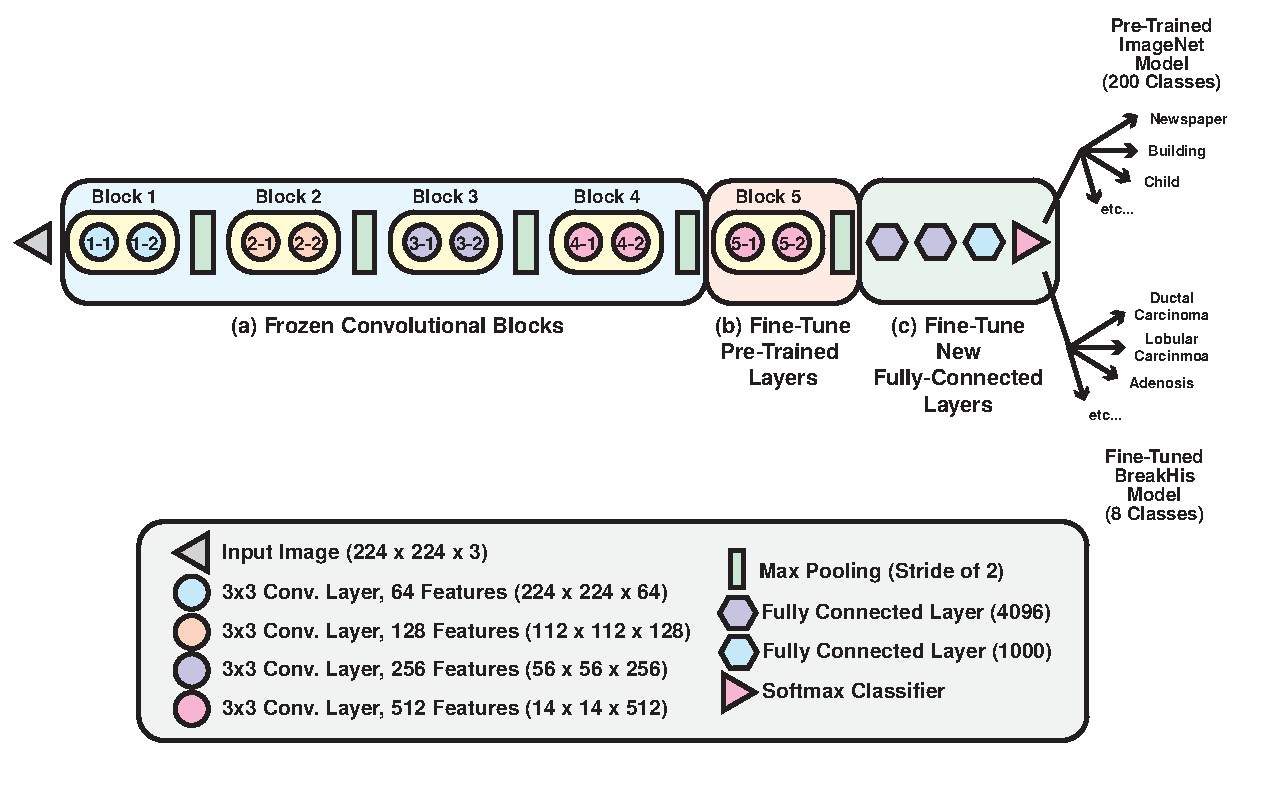
\includegraphics[width=160mm]{figures/deepduct/vgg_overview.pdf}
	\begin{singlespace}
		\textit{Legend} --- The VGG16 model is comprised of 16 weight layers, making up five convolutional blocks and a fully-connected classifier. Fine-tuning a pre-trained VGG16 model involves freezing the first four blocks (a), continuing to train the fifth block (b) against the new dataset (in this case, BreakHis) through backpropagation, and finally training a new fully-connected classifier against the new dataset (c).
	\end{singlespace}
	
\end{figure}
\section{Results}
\newpage
\section{Discussion}

% Summary of what you've done
The DeepDuct model described herein provides a proof-of-concept framework for the localisation of breast lesions from H\&E staining that does not rely on manual feature selection, transparently reports explanations for its predictions via class activation maps and allows for the potential discovery of new features that could inform future manual diagnosis.\par

% Why it's important
Neural networks have the advantage of dynamically ``learning'' and optimising features, as opposed to relying on a manual process of feature engineering that is often driven by limited powers of intuition and conventional knowledge. The automated process of feature engineering allows for the potential discovery of new underlying concepts previously not described in the literature that fundamentally define a class from others, and also prevents assumptions and misconceptions from biasing features and the resulting inaccuracies.\par

%Realising the impact that opaqueness has on the practicality of classifiers in these critical contexts, solutions have been created to provide insight and understanding regarding how models have arrived at their predictions, such as LIME and Grad-CAM \citep{}. To the author's understanding, DeepDuct is the first application of such technology to the classification and localisation of breast lesions from H\&E.
\subsection{Explanations for Neural Network Predictions are Essential for Clinical Use of CADe/x Models}

% How it stacks up to things other people have done
Whole-image ConvNet classification models fine-tuned on the BreakHis dataset have been previously described reporting high-accuracy, as well as patch-based whole-slide classifiers which apply whole-image classification to small patches of an imaged slide resulting, in a form of tumour localisation \citep{han2017, wang2016}. None of these models, however, offer the same extent of transparency and resolution offered by the activation maps provided by the Grad-CAM algorithm used in the DeepDuct model. Existing models of breast lesion classification and localisation remain ``black-box'' solutions to end-users, particularly those without in-depth knowledge of deep learning algorithms.\par

Unique among deep-learning based breast lesion classifiers, DeepDuct reports which regions of the input image have lead the model to classify the image as it had. This simultaneously allows for general localisation of classified objects and a glimpse into the internal state of the model, informing and not prescribing a diagnosis. This transparency is essential for a model to see use in contexts such as clinical settings where acting on predictions in blind faith is not an option due to the high-risk associated with the decisions being made. Models that implement ``explanations'' for their predictions have indeed been shown to increase end-user trust in model predictions, as well as help identify false-positive predictions made by a given model \citep{ribeiro2016}. To the author's understanding, DeepDuct is the first application of such explanatory algorithms to the classification and localisation of breast lesions from medical imaging.\par

% It's limitations
\subsection{Dataset Considerations}
\hl{subsection-needs-better-name}\\
The BreakHis dataset, while covering a number of relevant lesion types with a significantly large number of examples for each type, presents some important challenges. Firstly, despite the multiple magnifications provided, images in the BreakHis dataset are not of high-resolution, taken with a digital camera with pixel size of 6.5$\mathrm{\mu m}$ and resolution of 480 TV lines. Secondly, the number of examples is extremely imbalanced between classes, with as much of a 7.5-fold difference between the least represented class and the most represented class.\par

While low-resolution images can be useful for learning so-called ``global features'', they've proven to be problematic when distinguishing differences between objects with similar high-level features, as is the case between two H\&E images exhibiting different lesion subtypes. This problem is illustrated well in the description of Baidu's Deep Image model, whereby similar objects (such as insects of the same species) can only be distinguished from one another when higher-resolution images are considered in the model \citep{baidudeepimage}. Training the DeepDuct model on higher resolution datasets would address this concern. High-resolution datasets of breast lesions do exist, but many offer too few examples (INESCTC) or do not offer histological type information outside grade (CAMELYON16) \hl{citation-needed}.

As described early, imbalances in the number of examples provided per class in the BreakHis dataset had lead to a strong bias towards over-represented classes (\textit{Figure \ref{fig:confmat}a}). This bias was addressed by oversampling all under-represented classes by duplicating examples until all classes in the training set contained the same number of examples (\textit{Figure \ref{fig:confmat}b}).

\subsection{Future Directions \& Improvements}

Implementing the DeepDuct model on smartphones would afford clinicians low-cost, mobile tools for the annotated classification of breast histology slides through use of commercial or 3D-printable smartphone-microscope adapters \citep{cellphone_microscope_platform}. A less computationally-complex mobile DeepDuct implementation would be required to account for the limited resources available on the platform. This is typically achieved either by a networked server-client model supported by computation in the cloud, or by replacing the deep, resource-heavy VGG16 model with a more shallow mobile-oriented model such as SqueezeNet \citep{squeezenet}. While the former is limited by patient-privacy compliance and network connectivity, the latter requires retraining the network on a shallower ConvNet architecture with potential losses in accuracy.

Regional convolutional neural networks (R-CNNs), such as Facebook's Mask R-CNN, have been developed to provide pixel-resolution object detection in complex scenes \citep{mask_r_cnn}. Using a Mask R-CNN model trained on a breast lesion dataset can provide higher resolution lesion detection than existing patch-based breast lesion models \citep{wang2016}.

%The DeepDuct algorithm might also be combined with regional convolutional neural network (R-CNN) algorithms such as Mask to provide both explanations (in the form of Grad-CAM heatmaps) as well as per-pixel 

%Limited computational resources reduce the practicality of CADe/x such as DeepDuct which are based on convolutional neural networks. Reducing computational complexity can be achieved by using smaller, mobile-oriented architectures such as SqueezeNet.

% Improvements/Future Directions

%The automated nature of feature selection in neural networks can also pose challenges if the dataset is of low-quality or very small; as differences between classes that are present in the dataset, but do not reflect differences between the classes as a concept, can severely bias a model. This is epitomised by the parable of ``the tank problem'', whereby a neural network trained by the US government to identify concealed tanks was actually identifying dark skies as the images of tanks in the dataset were taken on a cloudy day \citep{dreyfus1992}. Errors such as these are mitigated by assuring datasets are large and representative of the variation of the population. \par

 

%results
%\chapter{Results}
\section{PPReCOGG: A Model for the Per-Pixel Classification of Early Breast Lesions via Gabor Features}

\subsection{PPReCOGG Classifies Sub-Regions of Perceptibly Distinct Textures in Synthetic Benchmarks}

To assess the baseline ability of the PPReCOGG model to distinguish natural patterns from one-another, the PPReCOGG model was trained and benchmarked against the Brodatz textures (namely the ``Raffia'' and ``Brick'' textures) compiled in the USC-SIPI image dataset, which is a common image dataset used in the evaluation of image processing and texture recognition community \citep{weber1997}. The brick and raffia textures were selected as they are visually distinct, and test images comprised of sub-regions of the two are perceptibly distinct upon visual inspection (\emph{Table 3.1a}).\par

Multidimensional scaling (MDS) embeddings allow us to project the forty-eight-dimensional Gabor energy features calculated from the Brick and Raffia Brodatz textures onto three dimensions (\emph{Figure \ref{embeddings}a}). These feature embeddings reveal that while they intersect, the feature space is divided into two distinct planes, each belonging to one of the two classes.

The PPReCOGG model achieved high average accuracy rates of 90\% in benchmarks consisting of the Raffia and Brick Wall Brodatz textures (\emph{Table 3.1}).\par


\begin{figure}[p]
	\begin{center}
	\caption{MDS Embedding of Gabor Energy Features from Brodatz and Early Human Breast Lesion Datasets \label{embeddings}}
	\end{center}
	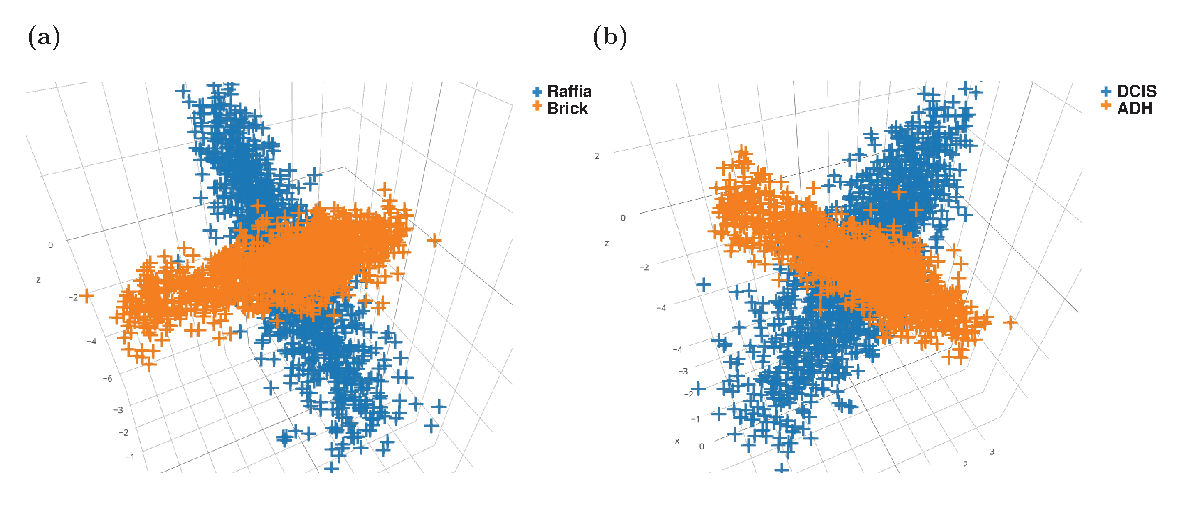
\includegraphics[width=170mm]{figures/embeddings/figure.pdf}
	 \begin{singlespace}
	 	\textit{Legend} --- Three-dimensional multidimensional scaling (MDS) embedding of Gabor energy features from known classes of the \textbf{(a)} Brodatz dataset and \textbf{(b)} the early human breast lesion dataset.
	 \end{singlespace}
	
\end{figure}


\clearpage

\begin{minipage}{\linewidth}
	\begin{center}
	
		\captionof{table}{Accuracy of the PPReCOGG Model Trained on Brodatz Textures 	\label{tab:brodatzclassify} }
		\begin{tabular}{>{\bfseries\centering}m{0.2in} >{\centering\bfseries}m{1in} >{\centering}m{1in} >{\centering}m{1in} >{\centering\arraybackslash}m{1in}}
			\hline
			&
			&
			\textbf{Test Image One}
			&
			\textbf{Test Image Two}
			&
			\textbf{Test Image Three}
			\\ 
			\hline
			(a)
			&
			Original
			&
			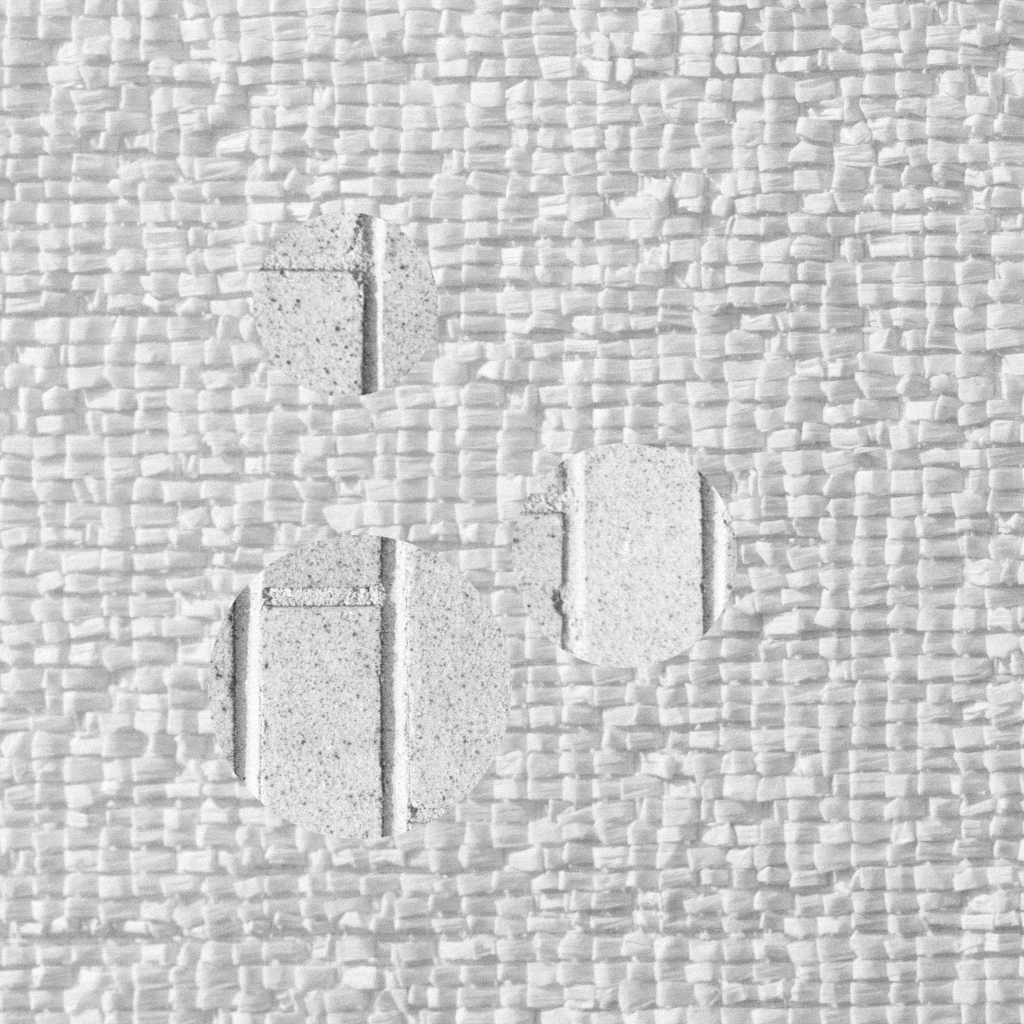
\includegraphics[width=75px, frame]{figures/accuracy_maps/original_brick_gravel_01.png}
			&
			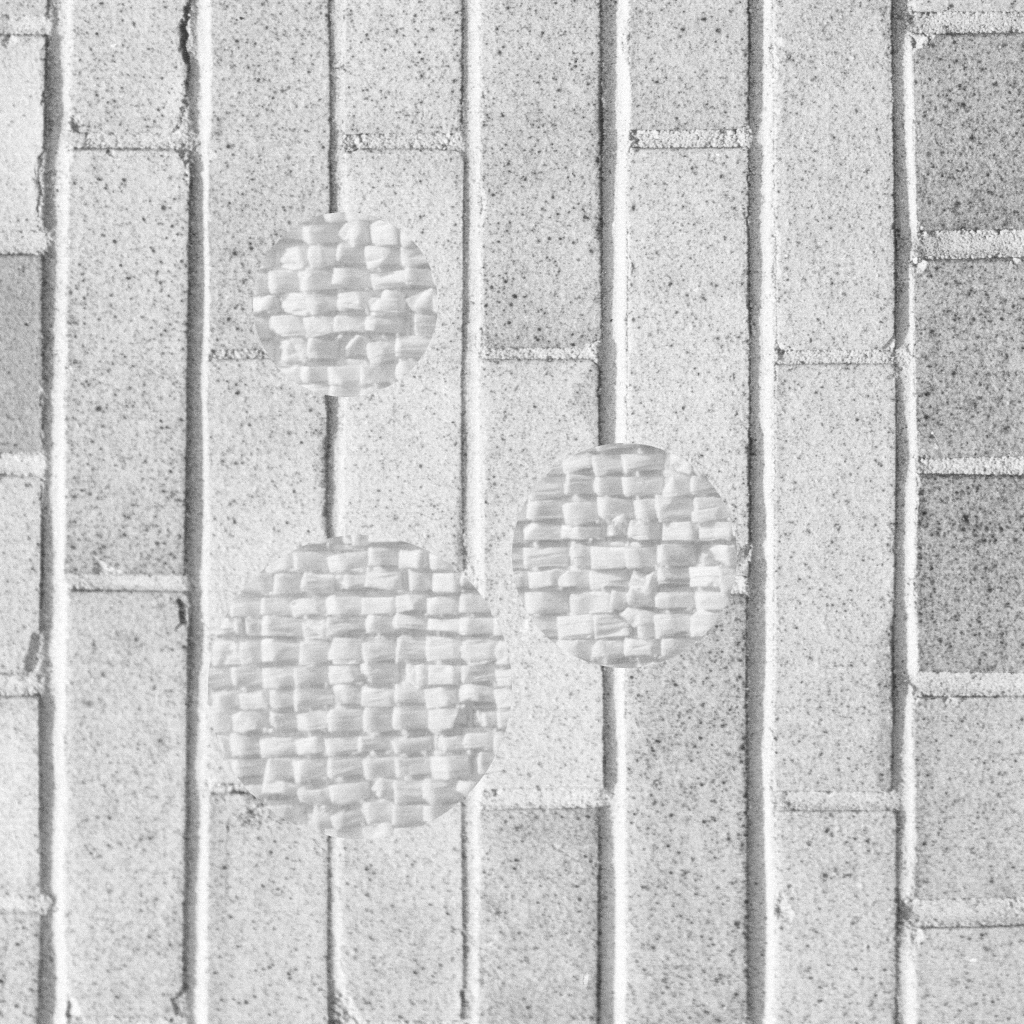
\includegraphics[width=75px, frame]{figures/accuracy_maps/original_brick_gravel_02.png}
			& 
			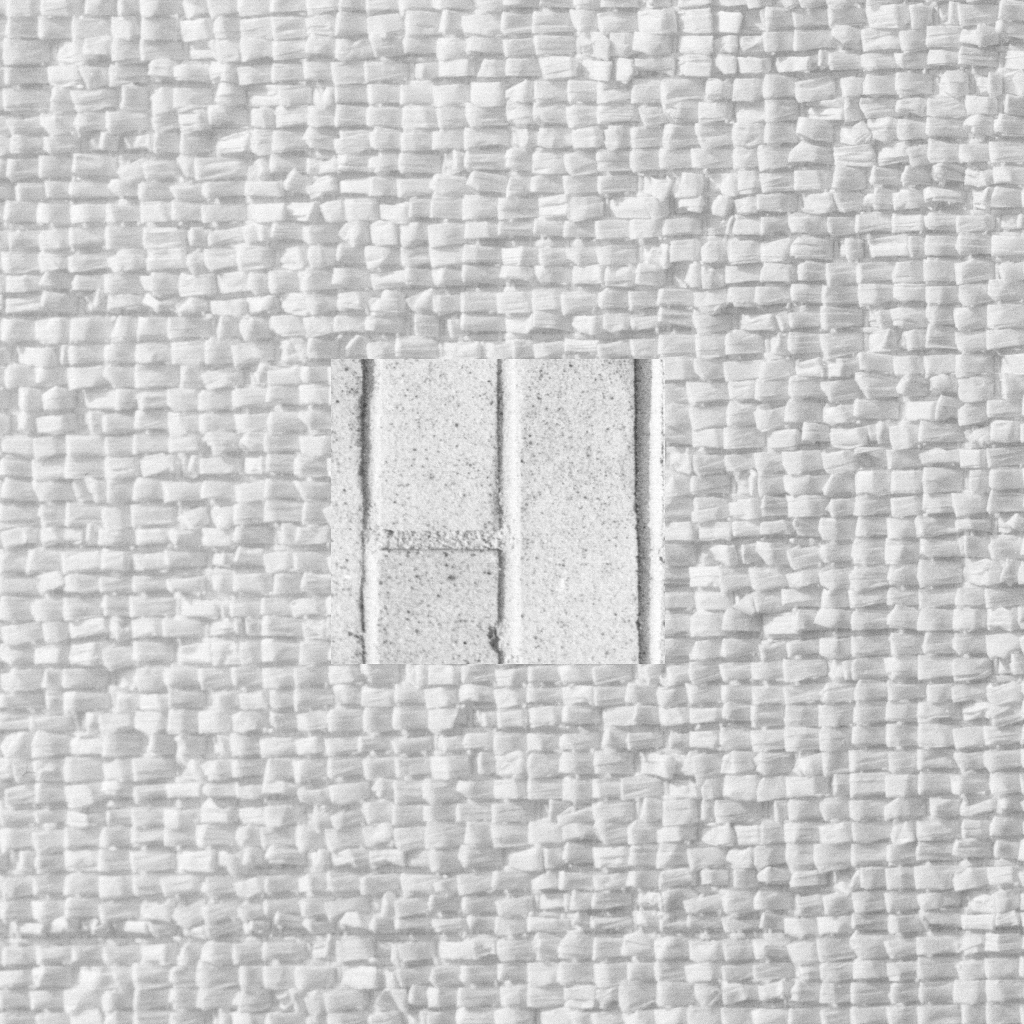
\includegraphics[width=75px, frame]{figures/accuracy_maps/original_brick_gravel_03.png}
			\\ 
			\hline
			(b)
			&
			Ground Truth
			&
			
\includegraphics[width=75px, frame]{figures/accuracy_maps/ground_truth_brick_gravel_01.png}
			&
			
\includegraphics[width=75px, frame]{figures/accuracy_maps/ground_truth_brick_gravel_02.png}
			& 
			
\includegraphics[width=75px, frame]{figures/accuracy_maps/ground_truth_brick_gravel_03.png}
			\\
			\hline
			(c)
			&
			Classified Image
			&
			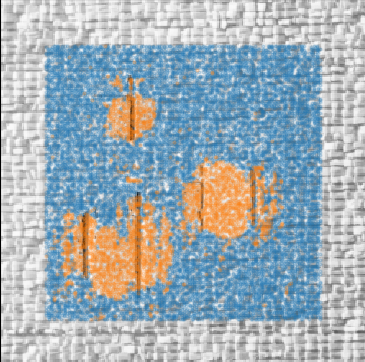
\includegraphics[width=75px, frame]{figures/accuracy_maps/brick_gravel_01_overlay_tight.png}
			&
			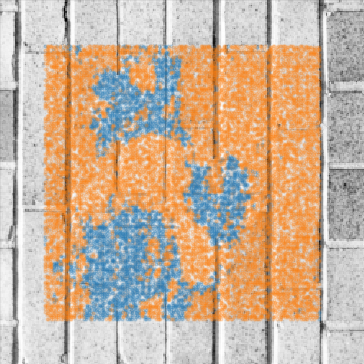
\includegraphics[width=75px, frame]{figures/accuracy_maps/brick_gravel_02_overlay_tight.png}
			&
			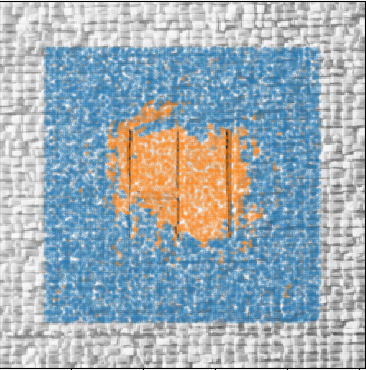
\includegraphics[width=75px, frame]{figures/accuracy_maps/brick_gravel_03_overlay_tight.png}
			\\
			\hline
			(d)
			&
			Raffia Accuracy Map
			&
			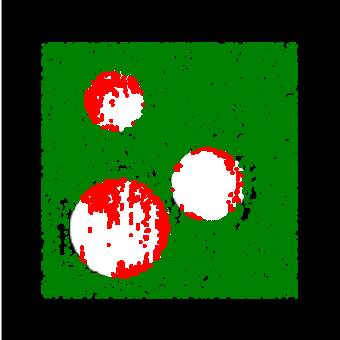
\includegraphics[width=75px, frame]{figures/accuracy_maps/brick_gravel_01_gravel_92_5.pdf}
			&
			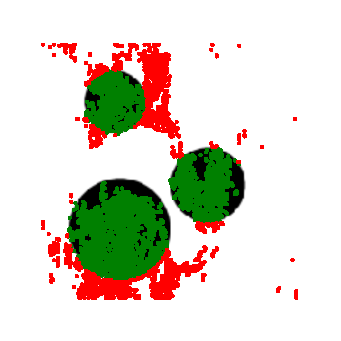
\includegraphics[width=75px, frame]{figures/accuracy_maps/brick_gravel_02_gravel.pdf}
			&
			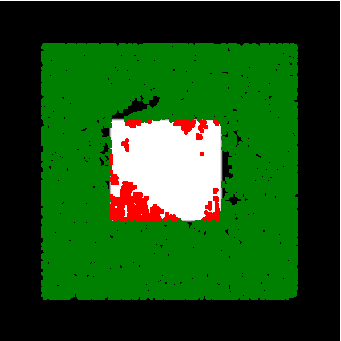
\includegraphics[width=75px, frame]{figures/accuracy_maps/brick_gravel_03_gravel.pdf}
			\\
			\hline
			(e)
			&
			Brick Accuracy Map
			&
			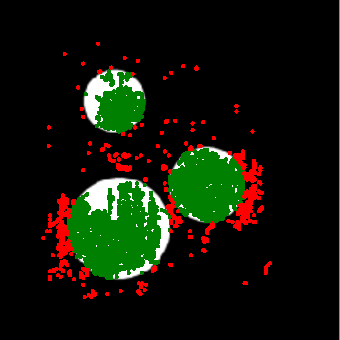
\includegraphics[width=75px, frame]{figures/accuracy_maps/brick_gravel_01_brick_84_6.pdf}
			&
			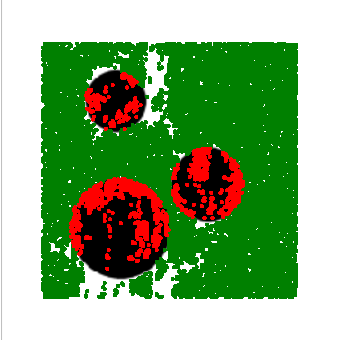
\includegraphics[width=75px, frame]{figures/accuracy_maps/brick_gravel_02_brick.pdf}
			&
			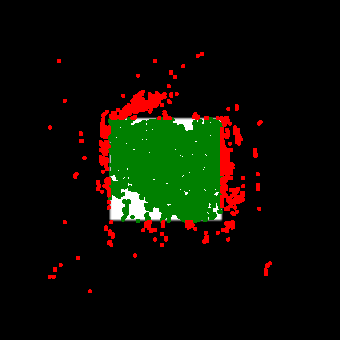
\includegraphics[width=75px, frame]{figures/accuracy_maps/brick_gravel_03_brick.pdf}
			\\ 
			\hline
			(f)
			&
			Accuracy
			&
			90.94\%
			&
			85.29\%
			&
			94.00\% 
			\\
			\hline
		\end{tabular}\par
	\end{center}
	\bigskip
	\begin{singlespace}
		\textit{Legend} --- \textbf{(a)} Test images comprised of composites of the Brodatz textures entitled ``Raffia'' (pg. D84) and ``Brick Wall'' (pg. D94). \textbf{(b)} The ideal classification (or ``ground truth'') of the original test image, where black pixels code for the raffia texture and white codes for the brick texture. \textbf{(c)} A random sampling of pixels classified by the PPReCOGG model. Pixels classified as Raffia are coded by blue points, and and pixels classified as Brick are coded by orange pixels. \textbf{(d)} and \textbf{(e)} Classified pixels are here compared to and overlayed on their ground truth. Pixels which are correctly classified are coded in green, while false-positives are coded in red. \textbf{(f)} Accuracy of the model, as calculated by the quotient of the number of correctly classified pixels and the total number of classified pixels. \label{brodatz_benchmark}
	\end{singlespace}
\end{minipage}



\subsection{PPReCOGG Classifies Sub-Regions of Different Neoplastic Phenotypes in Synthetic Benchmarks with High Accuracy}
\label{sec:synth_human}

Similar benchmarks were performed on test patterns composed of images of early lesions (ADH and DCIS) from human patient samples which had been immunofluorescently labelled for E-cadherin. These synthetic benchmarks are meant to simulate and quantitatively measure the efficiency of the PPReCOGG model in the task of classifying whole fields into sub-regions which exhibit cell patterning characteristic to certain early lesions.\par

MDS embeddings of the 48-dimensional Gabor energy features for the human samples reveal results very similar to the embeddings of the features of the Brodatz textures; two distinct but intersecting planes (\textit{Figure \ref{embeddings}b}).\par

The PPReCOGG model achieved high accuracy rates on the human lesion benchmarks, achieving an accuracies ranging from 93.17\% to 96.00\% across all test images (\textit{Table \ref{human_lesion}}).\par



\subsection{PPReCOGG Effectively Classifies Sub-Regions of Different Neoplastic Phenotypes in Human Biopsy Samples}

PPReCOGG model trained on E-cadhering patterning found in early breast lesion phenotypes (same features as those used in \S\ref{sec:synth_human}, see \textit{Figure \ref{fig:pprecogg_human_lesion}a}). This model was subsequently used to classify the pixels in images of early human breast lesions in with \mbox{E-cadherin} had been immunofluorescently labelled (\textit{Figure \ref{fig:pprecogg_human_lesion}b}). PPReCOGG effectively classifies sub-regions within the image that exhibit different cell-patterning characteristically found in early lesions.\par

\begin{minipage}{\linewidth}
	\begin{center}
		\label{tab:human_lesion} 
		\captionof{table}{Accuracy of the PPReCOGG Model Trained on Textures Derived from \mbox{E-cadherin} Staining of Human Lesions}
		\begin{tabular}{>{\bfseries\centering}m{0.2in} >{\centering\bfseries}m{1in} >{\centering}m{1in} >{\centering}m{1in} >{\centering\arraybackslash}m{1in}}
			\hline
			&
			&
			\textbf{Test Image One}
			&
			\textbf{Test Image Two}
			&
			\textbf{Test Image Three}
			\\ 
			\hline
			(a)
			&
			Original
			&
			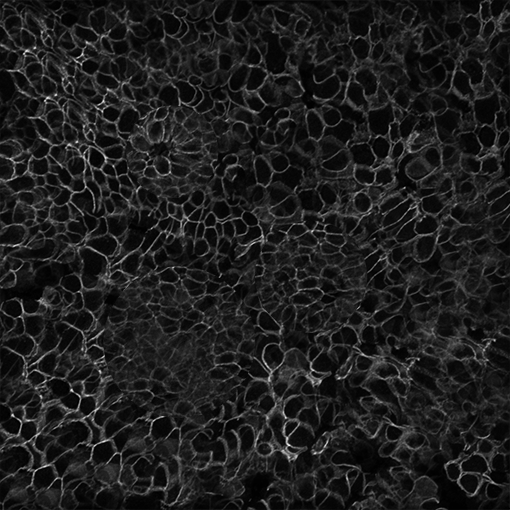
\includegraphics[width=75px, frame]{figures/accuracy_maps/if_fill/adh_dcis_01_dcis_bg.png}
			&
			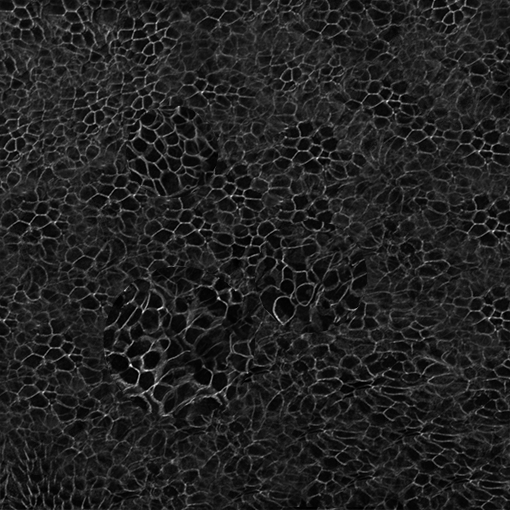
\includegraphics[width=75px, frame]{figures/accuracy_maps/if_fill/adh_dcis_02_adh_bg.png}
			& 
			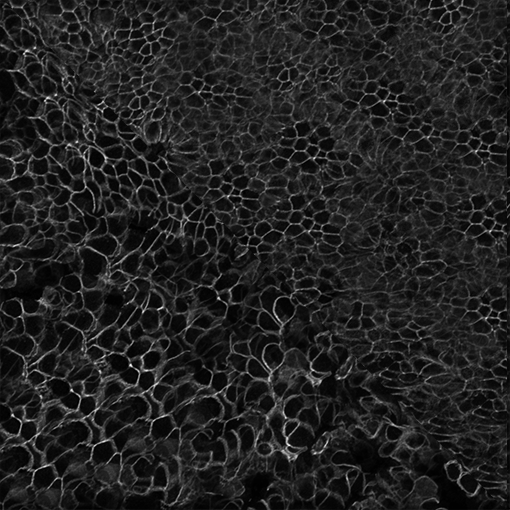
\includegraphics[width=75px, frame]{figures/accuracy_maps/if_fill/adh_dcis_02_adh_top_right.png}
			\\ 
			\hline
			(b)
			&
			Ground Truth
			&
			
\includegraphics[width=75px, frame]{figures/accuracy_maps/ground_truth_brick_gravel_01.png}
			&
			
\includegraphics[width=75px, frame]{figures/accuracy_maps/ground_truth_brick_gravel_02.png}
			& 
			
\includegraphics[width=75px, frame]{figures/accuracy_maps/if_fill/adh_dcis_510.png}
			\\
			\hline
			(c)
			&
			Classified Image
			&
			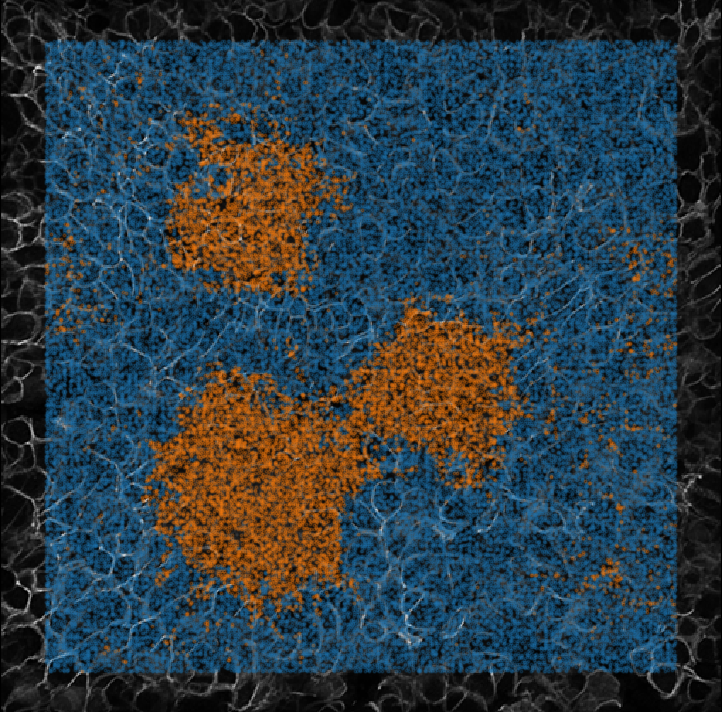
\includegraphics[width=75px, frame]{figures/accuracy_maps/if_fill/adh_dcis_classified_dcis_bg_tight.png}
			&
			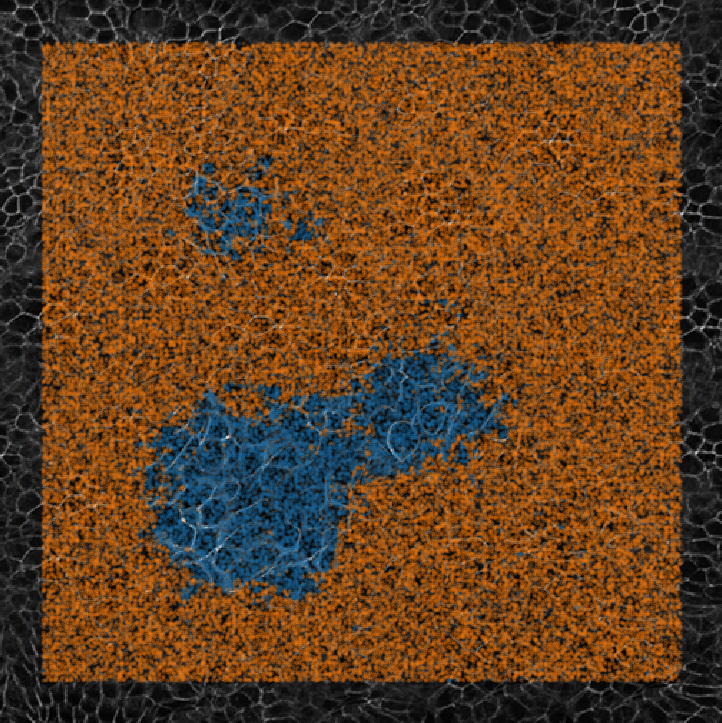
\includegraphics[width=75px, frame]{figures/accuracy_maps/if_fill/adh_dcis_classified_adh_bg_tight.png}
			&
			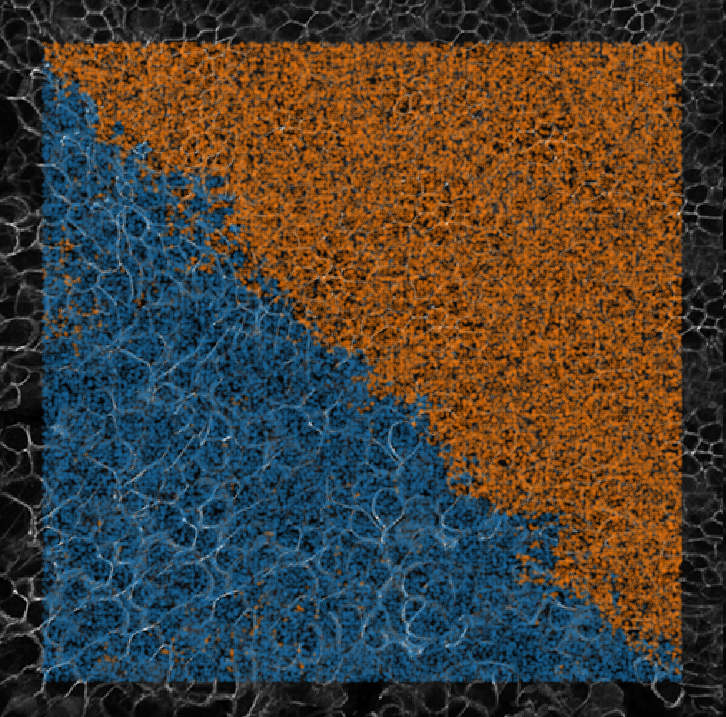
\includegraphics[width=75px, frame]{figures/accuracy_maps/if_fill/adh_dcis_slant_tight.png}
			\\
			\hline
			(d)
			&
			Hyperplasia Accuracy Map
			&
			\includegraphics[width=75px, frame]{figures/accuracy_maps/if_fill/accuracy_dcis_bg__adh_tight-01.pdf}
			&
			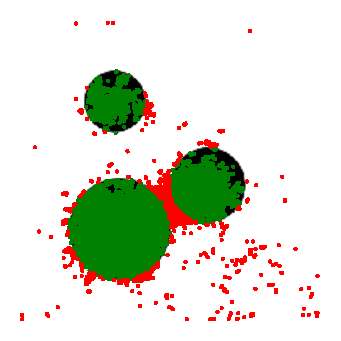
\includegraphics[width=75px, frame]{figures/accuracy_maps/if_fill/accuracy_adh_bg__dcis_tight-01.pdf}
			&
			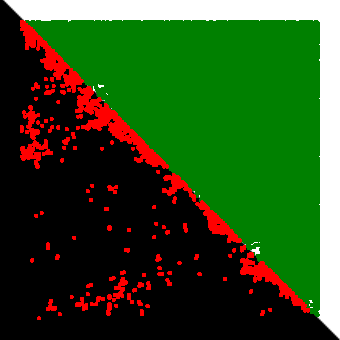
\includegraphics[width=75px, frame]{figures/accuracy_maps/if_fill/accuracy_slant_adh_bg__adh_tight-01.pdf}
			\\
			\hline
			(e)
			&
			Carcinoma Accuracy Map
			&
			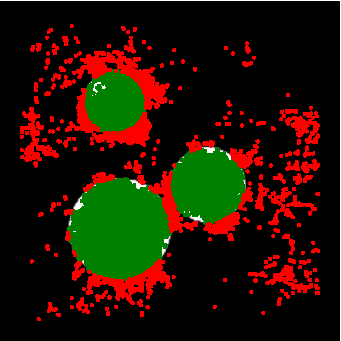
\includegraphics[width=75px, frame]{figures/accuracy_maps/if_fill/accuracy_dcis_bg__dcis_tight-01.pdf}
			&
			\includegraphics[width=75px, frame]{figures/accuracy_maps/if_fill/accuracy_adh_bg__adh_tight-01.pdf}
			&
			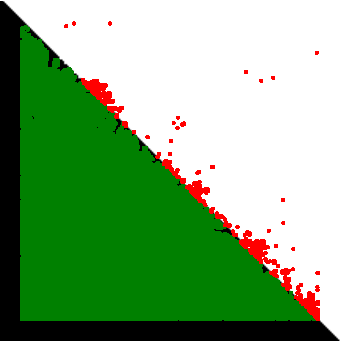
\includegraphics[width=75px, frame]{figures/accuracy_maps/if_fill/accuracy_slant_adh_bg__dcis_tight-01.pdf}
			\\ 
			\hline
			(f)
			&
			Accuracy
			&
			93.17\%
			&
			93.60\%
			&
			96.00\% 
			\\
			\hline
		\end{tabular}\par
	\end{center}
	\bigskip
	\begin{singlespace}
		\textit{Legend} --- \textbf{(a)} Test images comprised of composites of textures derived from \mbox{E-cadherin} staining of human lesions exhibiting characteristic hyperplastic or carcinomic cell patterning. \textbf{(b)} The ideal classification (or ``ground truth'') of the original test image, where black pixels code for the hyperplastic texture and white codes for the carcinomic texture. \textbf{(c)} A random sampling of pixels classified by the PPReCOGG model. Pixels classified as hyperplasia are coded by blue points, and and pixels classified as carcinoma are coded by orange pixels. \textbf{(d)} and \textbf{(e)} Classified pixels are here compared to and overlayed on their ground truth. Pixels which are correctly classified are coded in green, while false-positives are coded in red. \textbf{(f)} Accuracy of the model, as calculated by the quotient of the number of correctly classified pixels and the total number of classified pixels.
	\end{singlespace}
\end{minipage}



\begin{figure}[p]
	\begin{center}
		\caption{Human Lesions as Classified by the PPReCOGG Model \label{fig:pprecogg_human_lesion}}
	\end{center}
	\includegraphics[width=155mm]{figures/human_pprecogg.pdf}
	\begin{singlespace}
		\textit{Legend} --- Sections of human breast biopsies were immunofluorescently stained for E-cadherin and classified using the PPReCOGG model trained on two different early transformed phenotypes, and one background control. \textbf{(a)} Three representative fields of the 512 pixel by 512 pixel images used to train the PPReCOGG model. \textbf{(b)} Fields of breast E-cadherin labelled human breast lesion (left column) were classified by the trained \mbox{PPReCOGG} model (right column). Blue and orange pixels are classified as belonging to a hyperplastic carcinomic regions, respectively. Green pixels are classified as background signal.
	\end{singlespace}
	
\end{figure}

\section{DeepDuct: A Deep-Learning Approach to Regional Breast Cancer Classification using Grad-CAM}

\subsection{Accurate Classification of Breast Neoplasms in the BreakHis Dataset}

Transfer-learning the VGG16 on the unmodified BreakHis dataset results in acceptable overall classification accuracy (70\%), however closer inspection reveals bias towards one of the classes (ductal carcinoma) due to imbalances in the number of examples between classes (\emph{Figure \ref{fig:confmat}a}). Oversampling the dataset such that all classes have an equal number of training examples resulted in a small improvement in overall classification accuracy (72\%), and shows a demonstrable reduction in bias (\emph{Figure \ref{fig:confmat}b}).\par

Notably, lobular carcinomas were mistaken for ductal carcinomas in just over two-thirds of the validation set, and correctly identified a quarter of lobular carcinoma examples. After oversampling the BreakHis dataset, the accuracy and ductal carcinoma false-positive rates have nearly replaced one another, with lobular carcinomas being correctly classified in 63\% of cases and false ductal carcinoma classifications in a quarter of cases. Ductal carcinoma false-positives were in fact halved, on average, across nearly all classes after oversampling.\par

\subsection{Activation Mapping of BreakHis ConvNet using \mbox{Grad-CAM}}

The Grad-CAM algorithm was used to compute class activation maps from the BreakHis fine-tuned VGG16 ConvNet model (\emph{Figure \ref{fig:heatmap}}). In some cases, regions containing artefacts are highly activated and coincide with high-certainty (\textit{i.e.}: high predicted probability) false-positives (\emph{Figure \ref{fig:heatmap}e}). It is also not uncommon for low-certainty false-positives to be activated by similar regions across classes (\emph{Figure \ref{fig:heatmap}f}). Curiously, in many cases correct predictions are made that are largely activated by the stroma, rather than the epithelium (\emph{Figure \ref{fig:heatmap}c}).



\begin{figure}[p]
	\begin{center}
		\caption{Confusion Matrix of VGG16 Model Trained on the Original and Oversampled BreakHis Datasets \label{fig:confmat}}
	\end{center}
	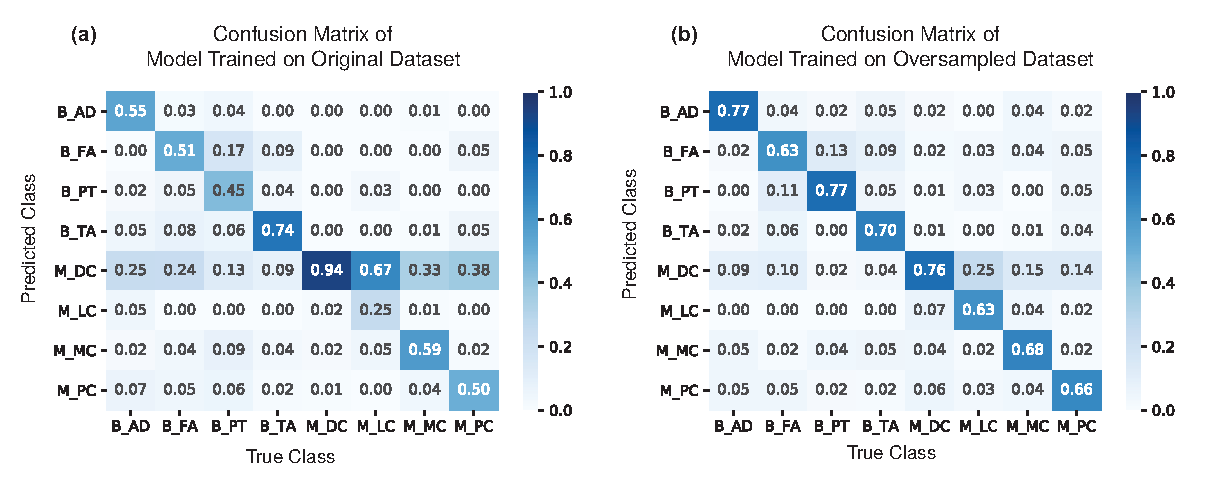
\includegraphics[width=170mm]{figures/deepduct/confusion_matrix.pdf}
	\begin{singlespace}
		\textit{Legend} --- Confusion matrices of the VGG16 model either trained on (a) the original BreakHis dataset as provided by its creators, or (b) a modified version of the BreakHis dataset oversampled such that each class has the same number of training examples. The model trained on the original dataset achieved an average accuracy of 70\% on the validation set across all classes, while the oversampled model saw a modest increase for a final average accuracy of 72\%. See Appendix A for class code legend used in this figure.
	\end{singlespace}
	
\end{figure}

\begin{figure}[t]
	\begin{center}
		\caption{Activation Maps of the BreakHis Fine-Tuned VGG16 ConvNet  \label{fig:heatmap}}
	\end{center}
	\includegraphics[width=150mm]{figures/deepduct/heatmaps.pdf}
	
	
\end{figure}
\begin{figure}[t]
	\begin{singlespace}
		\textit{Legend} --- Selected examples of activation maps of the BreakHis fine-tuned VGG16 model described herein, as calculated by the Grad-CAM algorithm. Column (i) displays the original input image and its ground truth classification. Column (ii) shows the top three predictions of the ConvNet and their activation maps overlayed on the input image; as well as the probability of the classification as reported by the model's softmax layer (shown in brackets). Column (iii) reports the probabilities of the top three predictions in a bar chart. Top probabilities are indicated with a checkmark (\ding{51}) when they match the ground truth (correct classification), and an ``x'' mark (\ding{55}) when they do not (false-positives). Rows (a--c) are examples of correct classifications made by the ConvNet model where the top prediction is of high probability. Rows (d--e) are examples of incorrect classification made by the ConvNet model where the top prediction is of high probability (false-positives). Row (f) is an example of an incorrect classification where none of the classes are reported to be of high-probability.
		
	\end{singlespace}
\end{figure}


%discussion
\chapter{Discussion}

%bibliography
\onehalfspacing
\bibliographystyle{authordate1}
\bibliography{references}
\inputencoding{utf8}
\chapter*{Appendix A: BreakHis Class Codes and Abbreviations}
\label{sec:class_codes}
\addcontentsline{toc}{chapter}{Appendix A: BreakHis Class Codes and Abbreviations}
\\
Abbreviations for the class names present in the BreakHis dataset are used throughout this manuscript, and within the model itself. These class names refer to the breast lesion types outlined in the WHO guidelines for the classification of breast tumours \citep{who_breast}.\par
\subsection*{Benign Tumours}
\begin{description}  
	\item [\texttt{B\_AD}] Benign Adenosis
	\item [\texttt{B\_FA}] Benign Fibroadenoma
	\item [\texttt{B\_TA}] Benign Tubular Adenoma
	\item [\texttt{B\_PT}] Benign Phylodes Tumour
\end{description}

\subsection*{Malignant Tumours}
\begin{description}  
	\item [\texttt{M\_DC}] Malignant Ductal Carcinoma
	\item [\texttt{M\_LC}] Malignant Lobular Carcinoma
	\item [\texttt{M\_MC}] Malignant Mucinous Carcinoma
	\item [\texttt{M\_PC}] Malignant Papillary Carcinoma
\end{description}
\newpage
\theendnotes

\end{document}